\documentclass{ose}
\usepackage{stfloats}
\usepackage{wrapfig}

%%% for HP squares in monster description
\makeatletter
\newcount\my@repeat@count
\newcommand{\repeatit}[3]{%
  % #1 = number of repetition
  % #2 = text to repeat
  % #3 = text in between
  \begingroup%
  #2%
  \my@repeat@count=\@ne%
  \@whilenum\my@repeat@count<#1\do{#2#3\advance\my@repeat@count\@ne}%
  \endgroup%
}
\newcommand{\oneHD}{{\small$\square\square\square\square\square\square\square\square$ }}
\newcommand{\hdsquares}[1]{\repeatit{#1}{\oneHD}{}}
\makeatother



\title{La tombe des rois serpents}

\begin{document}

\coverimage{pics/cover.png}
\maketitle
\thispagestyle{empty}

\tableofcontents

\chapter{Introduction}

Quand vous lancez Super Mario Bros. pour la première fois, le jeu ne vous donne aucune instruction.
Le premier niveau est savamment conçu pour vous enseigner les règles : sauter sur les ennemis, ramasser les champignons, trouver les secrets cachés, obtenir des pièces, éviter les trous.
Il n'y a pas de didacticiel.
Le jeu lui-même est le didacticiel.

Tout le monde peut citer des donjons "classiques" : Tomb of Horrors, La Barrière des Hautes Cimes, Ravenloft, etc.
Mais pour que ces aventures puissent prendre tout leur sens, une sorte d'introduction est nécessaire.
Tomb of Horrors et Death Frost Doom sont construits comme des réactions à un certain archétype de donjon, qui n'existe pas vraiment, pas sous forme de produit publié, tout du moins.

C'est comme si toutes les aventures à notre disposition étaient des compositions de Bach : les gens écrivent d'incroyables œuvres témoignant d'un génie incomparable, mais il faut que quelqu'un rédige un livre expliquant comment jouer du piano.

Ce donjon est conçu pour être "classique" sans pour autant être truffé de références ou empli de nostalgie.
Il se conforme à quelques clichés, mais pas tous. Il est également intégralement annoté.

\section{Ce module est destiné}
\begin{enumerate}
  \item Aux MJ expérimentés avec des joueurs débutants ;
  \item Aux MJ souhaitant apprendre à concevoir un donjon ;
  \item Aux MJ expérimentés avec des joueurs vétérans, mais découvrant l'OSR.
\end{enumerate}
Si vous êtes un MJ complètement débutant, vous pouvez toujours utiliser ce donjon et en apprendre beaucoup, mais il
mettra vos compétences à rude épreuve d'entrée de jeu.
Les joueurs expérimentés pourront probablement l'apprécier eux aussi.

\section{Je suis pas d'accord avec...}
Il y a de bonnes chances que les MJ expérimentés soient en désaccord avec certains pièges, leçons ou rencontres de ce
donjon.
Ce n'est pas un souci ! Ce module n'est pas censé être un guide de la "seule bonne façon" de mener un donjon
pour débutants, juste d'une des manières de procéder.

Si vous estimez que la diplomatie est une compétence vitale dès le début, ajoutez un gobelin amical mais froussard nommé
Smée au 7 : Faux Temple (p. 2).
Si vous pensez que les contraintes temporelles et le sentiment de danger imminent sont importants, faites intervenir des Monstres Errants à tous les niveaux du donjon, pas juste au troisième.
Si vous n'aimez pas les serpents, remplacez-les par des chèvres.
Ajoutez des clichés venus du folklore.
Remplacez les pièges par vos favoris, ou retirez-les complètement.

Au moins, en manifestant votre désaccord, vous apprenez à connaître vos propres préférences.
C'est toujours utile : savoir ce que l'on n'aime pas est aussi précieux que savoir ce que l'on
aime.
Qui sait ? Peut-être que ce module vous donnera l'envie d'écrire votre propre "donjon d'apprentissage"

\section{Taille du Groupe et Équilibre}
Ce donjon est conçu pour des personnages de niveau 1.
J'ai tenté le rendre aussi indépendant que possible de tout système de jeu.
Vous pouvez tout aussi bien mener ce donjon pour un joueur comme pour dix.
Les rencontres ne sont pas équilibrées.
Elles n'ont pas de "facteur de puissance".
Le combat n'est que peu récompensé, mais l'exécution réussie d'un bon plan l'est grandement.

La quantité de trésor est basée sur l'idée que 200 PO sont suffisants pour faire monter un personnage de niveau.
En arrivant au bout de ce donjon, les PJ survivants devraient avoisiner le niveau 2 voire 3, en supposant un taux standard d'attrition, perte et panique.
Ajustez la valeur du trésor en conséquence.
Les grands groupes auront moins de mal (et récupéreront moins de trésor par PJ).
Un joueur solo parvenant à survivre deviendra riche.

La puissance des coups est prévue pour des PJ ayant entre 4 et 16 points de vie, équipés de dagues causant 1d6 dégâts.
Les jets de sauvegarde sont décrits de façon générique (jet de sauvegarde contre le poison, pour esquiver...).

Un groupe de PJ de niveau moyen, joué par des joueurs expérimentés, pourrait venir à bout de ce donjon en un temps
record.
Il est tout de même possible qu'ils s'amusent.
Un groupe de PJ de bas niveau joué par des joueurs débutants devrait passer un très bon moment, du moins je l'espère.

En fonction du style de jeu, de la vitesse de progression, des aventures annexes, du temps passé en ville et autres digressions, l'exploration exhaustive de ce donjon peut se compléter en 12 à 24 heures de jeu.
La durée du Niveau 1 est adaptée à une courte première session précédée d'une création de personnages.

\section{Avant de Commencer}
\begin{enumerate}
  \item Lisez le module dans son intégralité.
  \item Prenez note de ce que vous aimez et n'aimez pas.
  \item Imprimez les pages 1 à 17 ainsi que la carte (p. III).
  \item Remplacez les monstres des pages 12 à 14 avec ceux du système choisi.
  \item Ajustez la valeur des trésors autant que nécessaire.
\end{enumerate}

\section{Appâter les PJ}
Voici quelques moyens d'amener les PJ au donjon, pour peu qu'ils soient sur la paille et qu'ils sachent que les tombes
contiennent souvent des trésors.
Vous pouvez placer ce donjon n'importe où.

\begin{enumerate}
  \item Ils trouvent une vieille carte menant à une sépulture tombée dans l'oubli.
  \item Un glissement de terrain révèle l'entrée de la tombe.
  \item Les gobelins (p. 13) kidnappent un proche des PJ.
  \item Les expériences de Xiximantre (p. 13) induisent en eux d'étranges rêves.
  \item Ils tombent sur l'entrée du tombeau alors qu'ils s'occupent d'un problème qui n'a rien à voir.
  \item Un puissant commanditaire les envoie explorer la tombe nouvellement découverte.
\end{enumerate}

\section{Leçons}
De petits encadrés didactiques sont parsemés au gré du texte.
Chaque salle, rencontre ou piège est conçu pour enseigner aux nouveaux joueurs (et nouveaux MJ) une leçon pertinente. Certaines d'entre elles sont d'ordre général, tandis que d'autres sont spécifiques à ce donjon.
La structure, la nature et les dangers du donjon deviennent peu à peu prévisibles et exploitables.
Les leçons peuvent paraître triviales aux MJ expérimentés, mais je pense que leur présence reste utile malgré
tout.

\section{Structure}
La Tombe des Rois Serpents est un donjon enterré divisé en trois niveaux et quatre zones thématiques.
J'ai inclus des descriptions minimales dans le texte et l'Index des Salles (p. 16).
Il n'y a pas de paragraphes "à lire à voix haute".

\subsection{Niveau 1 : La Fausse Tombe}
Introduit les bases de la conception et exploration de donjon en 7 salles.

Cette section est pile de la bonne longueur pour une première session, pourvu que la création de personnages ait été rapide et que vous ayez donné aux PJ une bonne raison d'explorer la tombe.

\subsection{Niveau 2 : La Tombe Supérieure}
Toujours linéaire, mais avec plus de pièces annexes et quelques dangers environnementaux.
Le chemin "vers l'avant" est toujours clair, mais les salles annexes sont tentantes.
C'est ici que les leçons du Niveau 1 sont évaluées et mises en pratique.

Cet étage devrait prendre 2 ou 3 sessions à explorer, et peut requérir un trajet de retour à la civilisation pour faire le plein.

\subsection{Niveau 3 : La Tombe Inférieure}
Il y a deux chemins principaux "horizontaux" et trois "verticaux".
Le donjon bifurque et reboucle.
Il est possible de remonter à la surface comme de plonger plus profond.
Ou même de revenir de là où l'on est parti.
Cet étage est indubitablement plus dangereux que les précédents.

La diplomatie et le troc font également leur apparition, de même que les monstres errants.
Vous pouvez explorer les niveaux 1 et 2 à votre rythme, mais passer trop de temps au Niveau 3 revient à prendre des risques inconsidérés.

La conclusion de cet étage est ouverte : vous pouvez ajouter du contenu pour étendre ce donjon autant que vous le souhaitez.
Arrivé là, si vous êtes un nouveau MJ ou débutant en jeux OSR, vous devriez être prêt à écrire votre propre donjon.

\section{Zones Thématiques}
\subsection{La Fausse Tombe}
Symbolise la joie de la découverte, le moment où l'on se dit "Oh ! Je vois !" et l'anticipation du trésor à venir.
Assurez-vous de féliciter tout joueur parvenant à déduire qu'il s'agit d'une fausse tombe : l'astuce se doit d'être récompensée.
Le donjon devient de plus en plus étrange au fur et à mesure de la descente.
Au début, on force des cercueils de bois pour voler de petites amulettes.
À la fin, on se retrouve à fouiller des déchets de gobelins fongiques pour trouver une couronne, à négocier avec un homme-serpent décédé, ou à convoyer des coffres d'or jusqu'à la surface.

Décrivez cette zone avec des mots comme "branlant", "décrépi" et "humide".
C'est une vieille cave.
De petites racines blanches pendent du plafond pour venir lécher le sol.

\subsection{La Vraie Tombe}
Représente le pouvoir et les menaces implicites.
Des statues veillent.
Des choses tressaillent dans leurs cercueils scellés.
Des lézards géants vous traquent dans l'obscurité, des sorciers immortels proposent des pactes indicibles et d'invincibles mucus morts-vivants serpentent à votre poursuite.

Décrivez cette zone avec des mots comme "énorme", "menaçant" et "froid".
C'est l'\oe uvre d'une civilisation bien plus ancienne, sage et cruelle que celle des PJ.
Plus ils s'enfoncent profondément, plus la tension devrait les rendre nerveux.

\subsection{Le Gouffre}
Incarne l'inconnu, et ses promesses.
Il pourrait y avoir n'importe quoi en bas.
Le centre de la Terre.
Des hommes-serpents vivant toujours paisiblement dans les profondeurs.
C'est la toile vierge du module, sur laquelle le MJ peut venir ajouter ce que bon lui semble.

Décrivez le gouffre avec des mots comme "sans fond", "vertigineux, comme si le monde entier s'écroulait" et "résonnant
de lointains mais persistants échos, si vous êtes patients".

Les PJ ne devraient pas vouloir passer plus de temps que nécessaire au bord de l'abîme.

\subsection{Les Terriers Gobelins}
Les Gobelins Fongiques sont le miroir des PJ, leur opposé.
Ils se complaisent dans la crasse, revivent sans cesse et commettent toujours les mêmes erreurs.
Ils sont affamés, stupides, superstitieux et meurtriers, mais néanmoins attachants.
Les terriers sont l'irruption d'un barbarisme bruyant et enthousiaste dans la civilisation froide et moribonde.

Décrivez les terriers tant par le bruit que par l'odeur.
Ça pue.
Vous allez puer si vous vous attardez ici, et la Tombe des Rois Serpents n'est pas pourvue de bains.
Des petits yeux de gobelins dans la pénombre.
Des dents cliquetantes et des couteaux aiguisés.

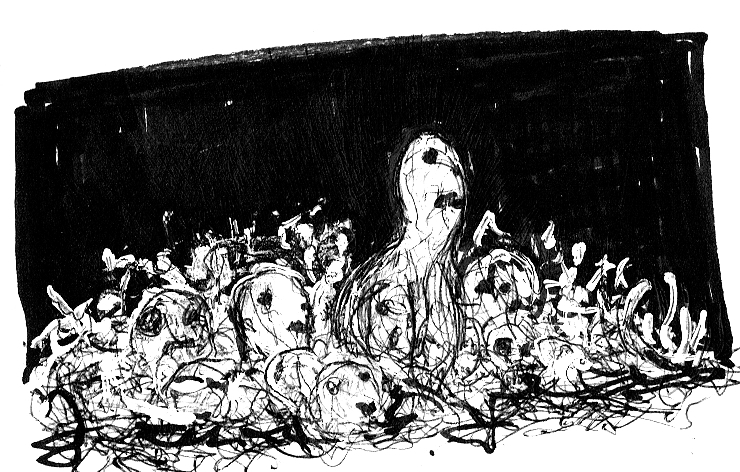
\includegraphics[width=\columnwidth]{pics/goblin_pit.jpg}
\chapter{Niveau 1 : La Fausse Tombe}
\section{Structure}
Cette section introduit les bases de la conception et exploration de donjon en 7 salles.

Elle est pile de la bonne longueur pour une première session, pourvu que la création de personnages ait été rapide et que vous ayez donné aux PJ une bonne raison d'explorer la tombe.

Elle symbolise la joie de la découverte, le moment où l'on se dit \emph{"Oh ! Je vois !"} et l'anticipation du trésor à venir.

Assurez-vous de féliciter tout joueur parvenant à déduire qu'il s'agit d'une fausse tombe : l'astuce se doit d'être récompensée.
\vfill
\pagebreak
\section{Description}
Décrivez cette zone avec des mots comme "branlant", "décrépi" et "humide".
C'est une vieille cave.
De petites racines blanches pendent du plafond pour venir lécher le sol.
\vfill
\pagebreak

\begin{figure}[hb]
  \centering
  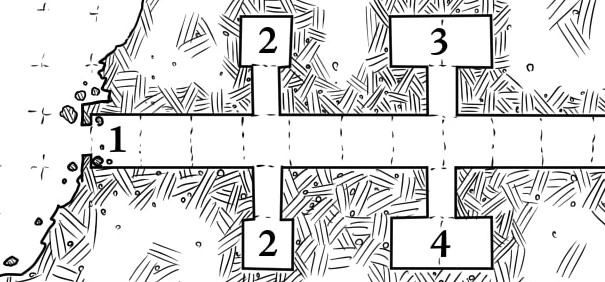
\includegraphics[width=\linewidth]{pics/map_1-4.jpg}
\end{figure}
\subsection{1 : Hall d’Entrée}\label{n1:s1}
\begin{itemize}
  \item 37m de long, sur 3m de large et 3m de haut.
  \item La lumière du soleil en atteint l’extrémité.
  \item Sent la \textbf{poussière}. Plus \textbf{froid} qu’à l’extérieur.
  \item Fines racines au plafond, \textbf{roche taillée grossièrement}
  \item 2 ouvertures de 1.5m de large chaque côté.
  \item Se termine par une porte barrée menant en \textbf{\nameref{n1:s6}}.
\end{itemize}

\subsection{2 : Tombes des Gardes}\label{n1:s2}
\begin{itemize}
  \item Salle de 3m sur 3m, 2.5m de haut
  \item Sent la \textbf{poussière} et le \textbf{vieux bois}, avec un léger \textbf{relent acide}.
  \item Roche taillée grossièrement, 
  \item Fresques de serpents entrelacés.
  \item Un \textbf{cercueil de bois} orné de gravures de scènes de bataille. Renferme :
  \begin{itemize}
    \item Statue de \emph{guerrier} en argile creuse, contient :
    \begin{itemize}
      \item une amulette d’or (10 PO)
      \item un squelette de serpent desséché
    \end{itemize}
    \item \textbf{Piège :} nuage de gaz empoisonné (Sauvegarde Poison ou 1d6 dégâts)
  \end{itemize}
\end{itemize}

\vfill\break
\subsection{3 : Tombe d’Érudit}\label{n1:s3}
\begin{itemize}
  \item Salle de 6m sur 3m, 2.5m de haut
  \item Sent la \textbf{poussière} et le \textbf{tissu putréfié}
  \item Roche taillée grossièrement
  \item Fresques de serpents bondissants.
  \item Un \textbf{cercueil de bois} orné de gravures abstraites, renferme :
  \begin{itemize}
    \item Statue d'\emph{érudit} creuse
    \begin{itemize}
      \item une amulette d’or (10 PO)
      \item un squelette de serpent desséché
    \end{itemize}
    \item Parchemins tombés en poussière
    \item \textbf{Piège :} nuage de gaz empoisonné (Sauvegarde Poison ou 1d6 dégâts)
  \end{itemize}
\end{itemize}

\subsection{4 : Tombe de Sorcier}\label{n1:s4}
\begin{itemize}
  \item Salle de 6m sur 3m, 2.5m de haut
  \item Sent la \textbf{poussière} et le \textbf{tissu putréfié}
  \item Roche taillée grossièrement
  \item Fresques de serpents bondissants.
  \item Un \textbf{cercueil de bois} orné de gravures macabres, renferme :
  \begin{itemize}
    \item Statue de \emph{sorcier} creuse
    \begin{itemize}
      \item une amulette d’or (10 PO)
      \item un squelette de serpent desséché
    \end{itemize}
    \item \textbf{Piège :} nuage de gaz empoisonné (Sauvegarde Poison ou 1d6 dégâts)
    \item Porte un anneau d’argent. Si arraché :
    \begin{itemize}
      \item Brise la statue
      \item Projette le poison
    \end{itemize}
  \end{itemize}
\end{itemize}

\begin{highlight}[Anneau d’argent]
  \begin{itemize}
    \item magique \textbf{et} maudit
    \item Porté au doigt, l’ongle s’allonge et bifurque en deux pointes aiguisées comme des crocs.
    \item Mêmes effet qu'une dague empoisonnée :
    \item Chaque matin  : Sauvegarde contre le poison ou 1d6 dégâts.
    \item Si 6 dégâts :  le doigt tombe et se transforme en serpent.
  \end{itemize}
\end{highlight}

%\begin{highlight}
%\textbf{Leçons :} Les trésors cachés peuvent être magiques, utiles et parfois maudits.
%\end{highlight}

\newpage
\subsection{5 : Porte / Marteau}\label{n1:s5}
Le corridor se termine par une \textbf{porte barrée}.
Deux pieux de fer plantés de chaque côté du chambranle soutiennent une lourde barre de pierre, bloquant l’accès à la salle suivante.

\begin{itemize}
  \item 3 PJ au moins pour la soulever
  \item \textbf{Soulevée :} Piège (Sauvegarde Mort ou 2d6+4 dégâts).
\end{itemize}

\begin{highlight}[Le piège]
  \begin{itemize}
    \item Marteau de pierre bascule du plafond
    \item Remplit \emph{presque} intégralement le couloir
    \item \textbf{\'Eviter :}
    \begin{itemize}
      \item Se plaquer au mur
      \item S'aider d'un autre PJ pour prendre appui : +2 au jet, -2 à l'autre PJ.
    \end{itemize}
    \item \textbf{Détection :}
    \begin{itemize}
      \item Examiner la porte, le plafond
      \item Examiner les pieux : se redressent lentement lorsque la barre est soulevée
    \end{itemize}
    \item \textbf{Désactiver :}
    \begin{itemize}
      \item Replacer la barre
      \item Maintenir les pieux en position basse
      \item Endommager le mécanisme au plafond
    \end{itemize}
  \end{itemize}
\end{highlight}

À moins que quelque chose ne le bloque, le marteau se rétracte lentement dans le plafond.

Il peut être activé à nouveau en abaissant les pieux de fer, à la main ou avec une corde.

L’impact force violemment l’ouverture des portes menant en \textbf{\nameref{n1:s6}}

\subsection{7 : Faux Temple}\label{n1:s7}
\begin{itemize}
  \item Salle de 6m sur 6m, 3m de haut
  \item Sent  fortement le \textbf{moisi},et la \textbf{pierre humide}
  \item \textbf{Statue d’un dieu homme-serpent}.
  \begin{itemize}
    \item Gigantesque, Hideux
  \end{itemize}
  \item Eau suinte du plafond
  \item L'eau a érodé le sol
  \item S'infiltre sous la statue :
  \begin{itemize}
    \item Révèle \textbf{\nameref{n2:s8}} vers le \textbf{\nameref{n2}} du donjon
  \end{itemize}
\end{itemize}
\vfill

\begin{center}
  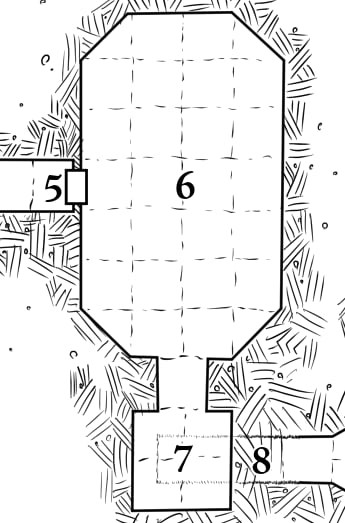
\includegraphics[width=\columnwidth]{pics/map_5-8.jpg}
\end{center}
\subsection{6 : Fausse Tombe Royale}\label{n1:s6}
La chambre funéraire du roi des hommes-serpents et ses deux épouses.
\begin{itemize}
  \item Salle de 12m sur 21m, 2.5m de haut
  \item Sent la \textbf{poussière}, \textbf{l’os} et le \textbf{moisi}
  \item Roche taillée grossièrement
  \item Fresques délitées de paysages.
  \item \textbf{3 cercueils de bois} long du mur nord
  \begin{itemize}
    \item Peints: hommes serpents endormis.
    \item Celui du milieu plus volumineux
    \item Contiennent chacun un \textbf{\nameref{monster:s6}}
    \item Attaquent dès que leur repos est troublé
  \end{itemize}
\end{itemize}



%\begin{highlight}
%\textbf{Leçons :} il y a des passages secrets.
%Ils sont associés aux statues.
%Il pourrait s’agir d’une fausse tombe.
%Tout au long de ce donjon, les statues sont synonymes de passages secrets et de trésors.
%\end{highlight}
\chapter{Niveau 2}\label{n2}

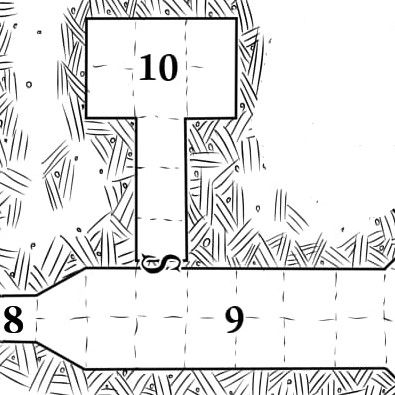
\includegraphics[width=\columnwidth]{pics/map_8-10.jpg}
\subsection{8 : Passage Secret}\label{n2:s8}
\begin{itemize}
  \item Directement sous \textbf{\nameref{n1:s7}}
  \item \'Etroite alcôve s’élargissant sur \textbf{\nameref{n2:s9}}
\end{itemize}

\subsection{9 : Hall aux Statues}\label{n2:s9}
Un long et large couloir. 
\begin{itemize}
  \item Six énormes sculptures d’hommes-serpents en armes et armures
  \item Regard dédaigneux
  \item $1^{ère}$ à gauche : légèrement désalignée
  \item  déplacée, révèle \textbf{\nameref{n2:s10}}
\end{itemize}

\vfill\break
\subsection{10 : Salle de Garde Secrète}\label{n2:s10}
Cette pièce fut autrefois une salle de garde secrète pour
les assassins du temple. 

\begin{itemize}
  \item Aujourd'hui vide et sombre. 
  \item Les meubles ont pourri jusqu’à se désagréger. 
  \item Deux guisarmes sont toujours utilisables
  \item Une icône religieuse en argent valant 50 PO.
\end{itemize}
\chapter{Niveau 3 : La Tombe Inférieure}\label{n3}
\section{Structure}
Il y a deux chemins principaux "horizontaux" et trois "verticaux".
Le donjon bifurque et reboucle.

Il est possible de remonter à la surface comme de plonger plus profond.
Ou même de revenir de là où l'on est parti.
Cet étage est indubitablement plus dangereux que les précédents.

La diplomatie et le troc font également leur apparition, de même que les \nameref{monster:n3:errants}.
Vous pouvez explorer les niveaux 1 et 2 à votre rythme, mais passer trop de temps au Niveau 3 revient à prendre des risques inconsidérés.

La conclusion de cet étage est ouverte : vous pouvez ajouter du contenu pour étendre ce donjon autant que vous le souhaitez.
Arrivé là, si vous êtes un nouveau MJ ou débutant en jeux OSR, vous devriez être prêt à écrire votre propre donjon.

\section{Zones Thématiques}
\subsection{Les Terriers Gobelins}
Les Gobelins Fongiques sont le miroir des PJ, leur opposé.
Ils se complaisent dans la crasse, revivent sans cesse et commettent toujours les mêmes erreurs.
Ils sont affamés, stupides, superstitieux et meurtriers, mais néanmoins attachants.
Les terriers sont l'irruption d'un barbarisme bruyant et enthousiaste dans la civilisation froide et moribonde.

Décrivez les terriers tant par le bruit que par l'odeur.
Ça pue.
Vous allez puer si vous vous attardez ici, et la Tombe des Rois Serpents n'est pas pourvue de bains.
Des petits yeux de gobelins dans la pénombre.
Des dents cliquetantes et des couteaux aiguisés.

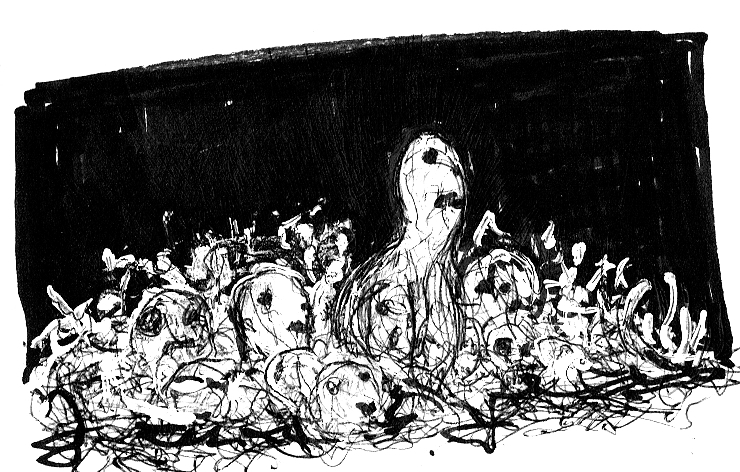
\includegraphics[width=\columnwidth]{pics/goblin_pit.jpg}

\vfill
\pagebreak
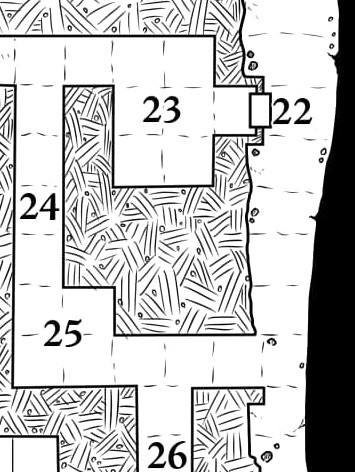
\includegraphics[width=\columnwidth]{pics/map_22-25.jpg}
\subsection{22 : Porte de Pierre}\label{n3:s22}
\begin{itemize}
  \item Enfoncée d’1,50m dans le mur
  \item Maintenue fermée par une lourde barre de pierre côté gouffre. 
  \item En arrivant par l’autre côté, la porte ne peut être ouverte sans être détruite.
  \item \textbf{Piège :}
  \begin{itemize}
    \item Même que \nameref{n1:s5}
    \item Marteau vers l’extérieur :
    \begin{itemize}
      \item 1D6 dommage \textbf{puis :} (sauvegarde contre la mort +2 annule) 
      \item Poussé dans le gouffre (sauvegarde contre la mort annule)
    \end{itemize}
  \end{itemize}
\end{itemize}

\subsection{24 : Couloir}\label{n3:s24}
\begin{itemize}
  \item Couloir de 3m sur 12m, 3m de haut
  \item Sent légèrement l'\textbf{acide}
  \item Bruits de \textbf{claquements humides}.
  \item Descend en pente douce vers le sud.
  \item \textbf{\nameref{monster:n3:squelgel}} au sud attiré par le bruit
\end{itemize}

\subsection{23 : Salle Cérémonielle}\label{n3:s23}
\begin{itemize}
  \item Salle de 6m sur 9m, 3m de haut
  \item Sent les \textbf{champignons séchés} et la \textbf{poussière}.
  \item Bancs au centre
  \item Anciennes tapisseries aux murs
  \item Fontaine asséchée (mur sud) : 
  \begin{itemize}
    \item Résidus d'or (10PO) sur espace plat au milieu
  \end{itemize}
\end{itemize}

Utilisée autrefois par les prêtres hommes-serpents pour se préparer et méditer. 

Les gobelins ont arraché la statue d’or qui ornait la fontaine pour la cacher dans leur salle du trône.

\subsection{25 : Fosse Piégée}\label{n3:s25}
\begin{itemize}
  \item Salle de 6m sur 6m, 3m de haut 
  \item Air \textbf{froid}
  \item Carrelage de dalles : 
  \begin{itemize}
    \item certaines cassées
    \item une manquante
  \end{itemize}
  \item \textbf{Piège :}
  \begin{itemize}
    \item Corniche large de 30 cm le long des murs \textbf{sûre}
    \item Autres carreaux ne sont soutenus que par de fines barres de métal
    \item Pied dans la zone centrale :
    \begin{enumerate}
      \item \textbf{Chute :} 1D6 dégâts (sauvegarde contre la mort annule)
      \item \textbf{Empalé} par les pics au fond : 1D6 dégâts (sauvegarde contre la mort annule)
    \end{enumerate}
  \end{itemize}
\end{itemize}

La fosse contient plusieurs squelettes d’humains normaux, ainsi qu’un anneau d’or valant 20 PO. 

Les gobelins remplacent les dalles chaque jour : ils utilisent le piège pour capturer leurs proies.

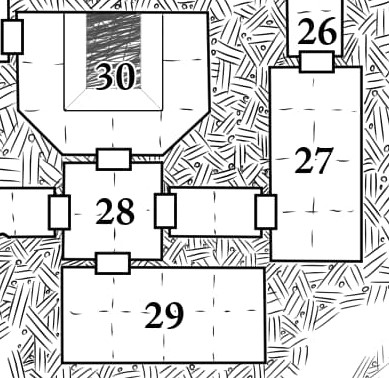
\includegraphics[width=\columnwidth]{pics/map_26-30.jpg}
\subsection{26 : Couloir}\label{n3:s26}
\begin{itemize}
  \item Couloir de 3m sur 6m, 3m de haut
  \item Mène à porte verrouillée :
  \begin{itemize}
    \item \textbf{Serrure aisée :} capacité voleur x2
    \item \textbf{Corrodée :} considérer comme une porte bloquée
  \end{itemize}
\end{itemize}

\subsection{27 : Salle des Esclaves}\label{n3:s27}
\begin{itemize}
  \item Salle de 6m sur 12m, haute de 3m
  \item Air \textbf{chaud et vicié}. 
  \item Taches de sang et roche usée
  \item \textbf{Sifflement} constant au sud-est.
  \item \textbf{Entraves rouillées} au sol.
  \begin{itemize}
    \item Se referment aux jambes si à moins de 30cm
    \item Rouille : Brisées avec test de force
  \end{itemize}
\end{itemize}

\vfill
\pagebreak
\subsection{28 : Dôme}\label{n3:s28}
\begin{itemize}
  \item Salle de 6m sur 6m, haute de 6m
  \item Air \textbf{chaud et vicié}. 
  \item \textbf{Sifflement} constant au nord.
  \item Plafond : \textbf{Dôme},  fresques d’hommes-serpents triomphants
  \item Porte au milieu de chaque mur.
  \item Porte sud verrouillée :
  \begin{itemize}
    \item Clef est au cou du Basilic (p. 14)
    \item Trop épaisse pour être brisée
  \end{itemize}
  \item Porte de pierre brisée à l’est. 
  \item Porte de pierre entrouverte vers le nord.
\end{itemize}

\subsection{29 : Salle du Trésor}\label{n3:s29}
\begin{itemize}
  \item Salle de 12m sur 6m, haute de 6m
  \item Contient tout ce que le MJ jugera bon de mettre au fond d’un donjon. [2000 PO au moins]
\end{itemize}

\subsection{30 : Fosse Sacrificielle}\label{n3:s30}
\begin{itemize}
  \item Salle de 12m sur 9m, haute de 6m
  \item Air vicié,
  \item \textbf{Flamme orangée} au nord, au fond d’une fosse profonde de 5m  aux parois en pente.
  \item Feu est alimenté par du gaz naturel acheminé depuis une antique mine perdue dans les tréfonds
  \item Chemin large de 60 cm borde le trou
  \item \textbf{Os carbonisés} couvrent le fond
  \item \textbf{Coulures d’or} sont visibles autour de la flamme 
  \item \textbf{Pierres précieuses} couvertes de carbone (500 PO en tout) scintillent dans la lueur orangée du feu
  \item Si PJ entrent dans la fosse :
  \begin{itemize}
    \item -1D6 CON (temporaire, sauvegarde poison annule)
    \item 0 CON : inconscient, glisse jusqu'à la flamme :  2d6 dégâts de feu par round
  \end{itemize}
\end{itemize}


\chapter{Description des monstres}
\section{Niveau 1}
\subsection{Squelette}\label{monster:s6}
\begin{itemize}
  \item \textbf{Apparence :} 
  \begin{itemize}
    \item Squelette humain muni de crocs et d’une arme rouillée. 
    \item Couvert de bracelets.
  \end{itemize}
  \item \textbf{ Désirs :} protéger le reste de la Tombe des Rois Serpents et tuer tout intrus.
\end{itemize}

\SetTblrInner{hspan=minimal, vspan=even}
\begin{osetable}{X[2]X[1]X[1]X[2]}{0}
  \SetCell[c=4]{bg=black,fg=white} {\bfseries\large\sectionfont Statistiques} & & &\\
  \textbf{CA}          & 7 [12] & \textbf{TACO}        & 19 [0] \\
  \textbf{Attaque}     & \SetCell[c=3]{l} 1D6 (griffes) & &\\
  \textbf{Sauvegardes} & \SetCell[c=3]{l} {\small \textbf{MP}~12 \textbf{B}~13 \textbf{PP}~14 \textbf{S}~15 \textbf{SSB}~16}& &\\
  \textbf{Mouvement} & 18m    & \textbf{Moral} & 12 \\
  \textbf{DV} & 1   & \textbf{XP} & 10 \\
  \textbf{PV} (\hspace*{20pt}) & \SetCell[c=3]{l}\noindent\hdsquares{1} & &\\
  \textbf{PV} (\hspace*{20pt}) & \SetCell[c=3]{l}\noindent\hdsquares{1} & &\\
  \textbf{PV} (\hspace*{20pt}) & \SetCell[c=3]{l}\noindent\hdsquares{1} & &\\
\end{osetable}

\begin{itemize}
  \item Ne subissent que la moitié des dégâts infligés par les armes perçantes ou tranchantes.
  \item Ils craquent et cliquettent, meurtriers et implacables
\end{itemize}


\vfill
%\pagebreak
\section{Niveau 2}
\subsection{Fragments de Momie}\label{monster:s11}
\begin{itemize}
  \item \textbf{Apparence :} 
  \begin{itemize}
    \item Bras noircis et décomposés
    \item Doigts acérés
  \end{itemize}
  \item \textbf{ Désirs :}  étrangler des choses, occire les vivants.
\end{itemize}

\SetTblrInner{hspan=minimal, vspan=even}
\begin{osetable}{X[2]X[1]X[1]X[2]}{0}
  \SetCell[c=4]{bg=black,fg=white} {\bfseries\large\sectionfont Statistiques} & & &\\
  \textbf{CA}          & 7 [12] & \textbf{TACO}        & 19 [0] \\
  \textbf{Attaque}     & \SetCell[c=3]{l} 1D6 (griffes) & &\\
  \textbf{Sauvegardes} & \SetCell[c=3]{l} {\small \textbf{MP}~12 \textbf{B}~13 \textbf{PP}~14 \textbf{S}~15 \textbf{SSB}~16}& &\\
  \textbf{Mouvement} & 18m    & \textbf{Moral} & 12 \\
  \textbf{DV} & 1*   & \textbf{XP} & 13 \\
  \textbf{PV} (\hspace*{20pt}) & \SetCell[c=3]{l}\noindent\hdsquares{1} & &\\
  \textbf{PV} (\hspace*{20pt}) & \SetCell[c=3]{l}\noindent\hdsquares{1} & &\\
\end{osetable}

\begin{itemize}
\item \textbf{Maladie :}
\begin{itemize}
  \item Maladie putrescente au toucher
  \item Guérison magique inefficace
  \item Guérison naturelle 10x plus longue
  \item Ne peut être éliminée que par magie
\end{itemize}
\item \textbf{Mort-vivant}
\begin{itemize}
  \item Silencieux. 
  \item Insensible aux effets affectant les créatures vivantes. 
  \item Immunisée contre les sorts affectant ou lisant l’esprit.
\end{itemize}
\end{itemize}

Ils se tortillent, grimpent votre corps et tentent de vous étrangler.

\vfill
\pagebreak

\subsection{Sparamantur}\label{monster:s13}
\begin{itemize}
  \item \textbf{Apparence :} 
  \begin{itemize}
    \item Squelette humain muni de crocs et d’une arme rouillée. 
    \item Couvert de bracelets.
  \end{itemize}
  \item \textbf{ Désirs :} protéger le reste de la Tombe des Rois Serpents et tuer tout intrus.
\end{itemize}

\SetTblrInner{hspan=minimal, vspan=even}
\begin{osetable}{X[2]X[1]X[1]X[2]}{0}
  \SetCell[c=4]{bg=black,fg=white} {\bfseries\large\sectionfont Statistiques} & & &\\
  \textbf{CA}          & 7 [12] & \textbf{TACO}        & 17 [2] \\
  \textbf{Attaque}     & \SetCell[c=3]{l} 1D8 (Hache de bataille) & &\\
  \textbf{Déplacement} & 18m    & \textbf{Moral} & 12 \\
  \textbf{Sauvegardes} & \SetCell[c=3]{l} {\small \textbf{MP}~12 \textbf{B}~13 \textbf{PP}~14 \textbf{S}~15 \textbf{SSB}~16}& &\\
  \textbf{Mouvement} & 18m    & \textbf{Moral} & 12 \\
  \textbf{DV} & 3   & \textbf{XP} & 35 \\
  \textbf{PV} (\hspace*{20pt}) & \SetCell[c=3]{l}\noindent\hdsquares{3} & &\\
\end{osetable}

\begin{itemize}
  \item Ne subit que la moitié des dégâts infligés par les armes perçantes ou tranchantes.
  \item Il craque et cliquette, meurtrier et implacable
\end{itemize}

\vfill
\pagebreak

\subsection{Pudding Noir (Franbinzar)}\label{monster:s14}
\begin{itemize}
  \item \textbf{Apparence :}  100 kg de mélasse noire
  \item \textbf{ Désirs :} Se nourrir.
\end{itemize}

\begin{osetable}{X[2]X[1]X[1]X[2]}{0}
 \SetCell[c=4]{bg=black,fg=white} {\bfseries\large\sectionfont Statistiques} & & &\\
 \textbf{CA}          & 6 [13] & \textbf{TACO}        & 15 [4] \\
 \textbf{Attaque}     & \SetCell[c=3]{l} 2D8 (toucher) & &\\
 \textbf{Sauvegardes} & \SetCell[c=3]{l} {\small \textbf{MP}~10 \textbf{B}~11 \textbf{PP}~12 \textbf{S}~13 \textbf{SSB}~14}& &\\
 \textbf{Mouvement} & 18m    & \textbf{Moral} & 12 \\
 \textbf{DV} &  5   & \textbf{XP} & 300 \\
 \textbf{PV} (\hspace*{20pt}) & \SetCell[c=3]{l}\noindent\hdsquares{5} & &\\
\end{osetable}

\begin{itemize}
  \item \textbf{Immunité :} Blessé uniquement par le feu, autres: dégâts temporaires
  \item \textbf{Division :} Les attaques qui ne sont pas liées au feu (y compris les sorts) provoquent la division du pudding. Chaque coup crée un nouveau pudding de 1 DV qui inflige 1d6 points de dégâts.
  \item \textbf{Corrosion :} Peut dissoudre le bois ou le métal en un tour (10\% de chances).
  \item \textbf{Collant :} Peut se déplacer sur les murs et les plafonds.
  \item \textbf{Suintement :} Peut s’infiltrer à travers les petits trous et fissures.
  \item \textbf{Régénération :} Si tué, se régénère en 1d20 heures, à moins d’être incinéré.
  \item \textbf{Attaques multiples :} Peut cibler tous les PJ adjacents à chaque round, effectuant un jet d’attaque classique pour chacun.
\end{itemize}

Franbinzar était le dernier roi de la forteresse.

Sa momification ne s’est pas déroulée correctement.
Il s’est transformé en Pudding Noir.

On peut apercevoir 200PO d’anneaux noyés dans sa masse.

\vfill
\pagebreak

\subsection{Gardien Cobra de Pierre}\label{monster:s19}
\begin{itemize}
  \item \textbf{Apparence :} 
  \begin{itemize}
    \item  Chevalier de pierre vêtu d’une armure sculptée. 
    \item Une de ses mains manie une imposante épée dentelée.
    \item L’autre est libre au début du combat.
  \end{itemize}
  \item \textbf{ Désirs :}  protéger le reste de la Tombe des Rois Serpents et  tuer les intrus.
\end{itemize}

\begin{osetable}{X[2]X[1]X[1]X[2]}{0}
  \SetCell[c=4]{bg=black,fg=white} {\bfseries\large\sectionfont Statistiques} & & &\\
  \textbf{CA}          & 3 [16] & \textbf{TACO}        & 15 [4] \\
  \textbf{Attaque}     & \SetCell[c=3]{l} 2D6 (épée dentelée) & &\\
  \textbf{Sauvegardes} & \SetCell[c=3]{l} {\small \textbf{MP}~10 \textbf{B}~11 \textbf{PP}~12 \textbf{S}~13 \textbf{SSB}~14}& &\\
  \textbf{Mouvement} & 18m    & \textbf{Moral} & 12 \\
  \textbf{DV} &  4+1   & \textbf{XP} & 125 \\
  \textbf{PV} (\hspace*{20pt}) & \SetCell[c=3]{l}\noindent\hdsquares{4}~$\square$ & &\\
\end{osetable}

\textbf{Attaques :} Chaque round, le Gardien Cobra de Pierre peut
appliquer une de ces stratégies :
\begin{enumerate}
  \item \textbf{Appel du Bouclier :} 
  Le Gardien appelle à lui un des boucliers couvrant les murs de l’arène.
  \begin{itemize}
    \item 1d6 dégâts (jet de sauvegarde contre la mort pour esquiver) si sur trajectoire
    \item Garde le bouclier (+1 CA)
  \end{itemize}
  \item \textbf{Bond et Impact :} 
  Le Gardien bondit à travers les airs puis plonge jusqu’à 6 m de sa position initiale.
  \begin{itemize}
    \item toute créature adjacente : 1d4 dégâts (sauvegarde contre la mort annule). 
    \item si dégât : projeté au sol
  \end{itemize}
  \item \textbf{Attaque normale}
\end{enumerate}

\textbf{Stratégies possibles :}
\begin{itemize}
  \item Prendre le Gardien en \textbf{tenaille}
  \item \textbf{Fuir :} Trop imposant pour l'escalier
  \item \textbf{Courir :} suit le PJ tant que détectables
\end{itemize}

\section{Niveau 3}
\subsection{Monstres Errants}\label{monster:n3:errants}
\begin{enumerate}
  \item \textbf{Présage du Basilic.} 
  Des cliquetis et grincements d’une chaîne distante traînée sur de la roche et dans la poussière.
  \item \textbf{Présage de Gelées Squelettes.} 
  Des bruits de succion résonnant dans le lointain.
  \item \textbf{Présage de Gobelins.} 
  \begin{itemize}
    \item Chuchotis, gloussements, grincements de dents et pourléchage de babines. 
    \item Le reflet d’yeux rouges dans l’obscurité. 
    \item Un fumet de pourriture fongique.
  \end{itemize}  
  \item \textbf{Chauve-souris.} 
  Nullement hostile, mais effrayante sur le moment. 
  Volette de-ci de-là, plane en direction du gouffre.
  \item \textbf{\nameref{monster:n3:araignee}} 
  \item \textbf{1d6 \nameref{monster:n3:gob}} en reconnaissance. 
  \begin{itemize}
    \item 1d6 autres gobelins fongiques postés au détour du prochain couloir.
  \end{itemize}
  \item  \textbf{1 \nameref{monster:n3:squelgel}.}
  \item  \textbf{1d10+5 \nameref{monster:n3:gob}} parés au combat. 
  L’un d’eux est muni d’une lance faite de couverts, absurdement peu pratique à manier (1d6 dégâts, allonge)
\end{enumerate}

\vfill
\pagebreak
\subsection{Grosse Araignée}\label{monster:n3:araignee}
  \begin{itemize}
  \item De la taille d’un poing.
  \item Cherche à manger des chauves-souris, pas les PJ.
  \item \textbf{Venimeuse : } 1d4 dégâts (sauvegarde poison annule) 
  \item \textbf{lâche}
  \item Mets de choix pour les gobelins fongiques.
\end{itemize} 

\SetTblrInner{hspan=minimal, vspan=even}
\begin{osetable}{X[2]X[1]X[1]X[2]}{0}
  \SetCell[c=4]{bg=black,fg=white} {\bfseries\large\sectionfont Statistiques} & & &\\
  \textbf{CA}          & 7 [12] & \textbf{TACO}        & 19 [0] \\
  \textbf{Attaque}     & \SetCell[c=3]{l} 1D3 (morsure) + poison & &\\
  \textbf{Sauvegardes} & \SetCell[c=3]{l} {\small \textbf{MP}~12 \textbf{B}~13 \textbf{PP}~14 \textbf{S}~15 \textbf{SSB}~16}& &\\
  \textbf{Mouvement} & 9m    & \textbf{Moral} & 8 \\
  \textbf{DV} & 1/2   & \textbf{XP} & 5 \\
  \textbf{PV} (\hspace*{20pt}) & \SetCell[c=3]{l}\noindent$\square\square\square\square$ & &\\
\end{osetable}

\subsection{Gobelins Fongiques}\label{monster:n3:gob}
\SetTblrInner{hspan=minimal, vspan=even}
\begin{osetable}{X[2]X[1]X[1]X[2]}{0}
  \SetCell[c=4]{bg=black,fg=white} {\bfseries\large\sectionfont Statistiques} & & &\\
  \textbf{CA}          & 6 [13] & \textbf{TACO}        & 19 [0] \\
  \textbf{Attaque}     & \SetCell[c=3]{l} 1D6 (arme) & &\\
  \textbf{Sauvegardes} & \SetCell[c=3]{l} {\small \textbf{MP}~14 \textbf{B}~15 \textbf{PP}~16 \textbf{S}~17 \textbf{SSB}~18}& &\\
  \textbf{Mouvement} & 18m    & \textbf{Moral} & 7 \\
  \textbf{DV} & 1-1   & \textbf{XP} & 5 \\
  \textbf{PV} (\hspace*{20pt}) & \SetCell[c=3]{l}\noindent\hdsquares{1} & &\\
  \textbf{PV} (\hspace*{20pt}) & \SetCell[c=3]{l}\noindent\hdsquares{1} & &\\
  \textbf{PV} (\hspace*{20pt}) & \SetCell[c=3]{l}\noindent\hdsquares{1} & &\\
  \textbf{PV} (\hspace*{20pt}) & \SetCell[c=3]{l}\noindent\hdsquares{1} & &\\
  \textbf{PV} (\hspace*{20pt}) & \SetCell[c=3]{l}\noindent\hdsquares{1} & &\\
  \textbf{PV} (\hspace*{20pt}) & \SetCell[c=3]{l}\noindent\hdsquares{1} & &\\
  \textbf{PV} (\hspace*{20pt}) & \SetCell[c=3]{l}\noindent\hdsquares{1} & &\\
\end{osetable}

\begin{itemize}
  \item \textbf{Apparence :} 
  \begin{itemize}
    \item pâles et rabougris, 
    \item \'Enorme tête ovale
    \item Plein de dents et deux petits yeux rouges beaucoup trop près l’un de l’autre. 
    \item Texture évoque une purée de pommes de terre à la colle blanche. 
    \item Portent sur eux des couverts de  table.
  \end{itemize}
  \item \textbf{ Désirs :} un roi, à manger, des choses qui brillent, encore à manger
  \item \textbf{Non hostiles :} ils cherchent seulement à couronner quelqu’un Roi des Gobelins (Initialement)
  \item \textbf{Dialecte :} gobelin cliquetant et limité.
  \item Aisément \textbf{corruptibles}
  \item Si PJ hostiles:
  \begin{itemize}
    \item \textbf{Fuite}
    \item \textbf{Embuscades} récurrentes
    \item Sournois et patients
    \item Escaladent (lentement) les murs : surprendre les aventuriers en leur plongeant dessus
    \item Seaux d’eau pour éteindre les torches
    \item Cordes pour emmêler les combattants
    \item Tirent profit des pièges du donjon
    \item De nuit, harcèlent le campement
  \end{itemize}
\end{itemize}

Ils suivent loyalement leur roi jusqu’à la pleine lune, puis l’assaillent, le traînent jusqu’à un autel au sommet d’une colline et l’éventrent. 

Ils tentent d’avertir le groupe au sujet du Basilic (p. 14), mais ignorent l’existence du 39 : Passage Secret (p. 9) et ne connaissent rien des niveaux supérieurs : le Gardien Cobra de Pierre leur empêche d’y accéder. 

La nuit venue, ils utilisent les 41 : Escaliers vers la Surface (p. 9) pour se faufiler jusqu’à l’extérieur. 

À moins que la 48 : Fosse de Génération de Gobelins (p. 11) ne soit incendiée, le nombre de gobelins dans le donjon sera toujours "beaucoup trop de gobelins". 
Les gobelins fongiques sont des rats de laboratoire parvenus à s’échapper.

Bien que Xiximantre (p. 13) ne s’oppose pas à ce qu’on les lui rende, ils ne lui sont pas d’une grande utilité.

\subsection{Gelée Squelette}\label{monster:n3:squelgel}
\begin{itemize}
  \item \textbf{Apparence :} Un squelette couvert de mucus orange
  \item \textbf{ Désirs :}  écraser des crânes et créer plus de gelées squelettes.
\end{itemize}

\SetTblrInner{hspan=minimal, vspan=even}
\begin{osetable}{X[2]X[1]X[1]X[2]}{0}
  \SetCell[c=4]{bg=black,fg=white} {\bfseries\large\sectionfont Statistiques} & & &\\
  \textbf{CA}          & 7 [12] & \textbf{TACO}        & 19 [0] \\
  \textbf{Attaque}     & \SetCell[c=3]{l} 1D4 (griffes) & &\\
  \textbf{Sauvegardes} & \SetCell[c=3]{l} {\small \textbf{MP}~12 \textbf{B}~13 \textbf{PP}~14 \textbf{S}~15 \textbf{SSB}~16}& &\\
  \textbf{Mouvement} & 9m    & \textbf{Moral} & 12 \\
  \textbf{DV} & 2   & \textbf{XP} & 20 \\
  \textbf{PV} (\hspace*{20pt}) & N.A. & &\\
  \textbf{PV} (\hspace*{20pt}) & N.A. & &\\
  \textbf{PV} (\hspace*{20pt}) & N.A. & &\\
  \textbf{PV} (\hspace*{20pt}) & N.A. & &\\
\end{osetable}

\begin{itemize}
  \item Immunisés à tous dommages.
  \item \textbf{Solutions possibles:}
  \begin{itemize}
    \item Fuir, 
    \item les faire pétrifier par le Basilic (p. 14), 
    \item les précipiter dans le gouffre, 
    \item les attacher
    \item les enfermer dans une salle
    \item les précipiter en 25 : Fosse Piégée (p. 6) ou 37 :  Fosse Piégée (p. 9)
  \end{itemize}
\end{itemize}

Il y a 4 gelées squelettes dans le donjon. 
Si le groupe les immobilise toutes les 4, retirez-les de la \textbf{Table des \nameref{monster:n3:errants}}. 

Au bout d’un certain temps, ils finiront toujours par sortir des fosses et se libérer des cordes. 

Toute créature vivante tuée par une gelée squelette se transforme en une nouvelle gelée squelette en 10 minutes. 
Les gobelins fongiques sont immunisés.

\end{document}